\documentclass[10pt,a4paper]{article}

\usepackage[a4paper,margin=1.6cm]{geometry}
\usepackage[T1]{fontenc}
\usepackage{lmodern}
\usepackage{microtype}
\usepackage{amsmath}
\usepackage{graphicx}
\usepackage{booktabs}
\usepackage{tabularx}
\usepackage{enumitem}
\usepackage{caption}
\usepackage{titlesec}
\usepackage[hidelinks]{hyperref}

% Compact, easy-to-scan layout.
\setlist{nosep, leftmargin=*}
\titleformat*{\section}{\large\bfseries}
\titleformat*{\subsection}{\normalsize\bfseries}
\titlespacing*{\section}{0pt}{1.1ex}{0.5ex}
\titlespacing*{\subsection}{0pt}{0.8ex}{0.3ex}
\captionsetup{font=small, labelfont=bf, skip=3pt}
\setlength{\parindent}{0pt}
\setlength{\parskip}{0.5ex}
\newcommand{\code}[1]{\texttt{#1}}

\begin{document}

\begin{center}
  {\Large\bfseries OpenAI Gym Code Report}\\[3pt]
  Time-Aware Reinforcement Learning for Ball Catching under Visual Delay\\[2pt]
  ME5418 Group 30
\end{center}

%==========================================================================================
\section{Code Explanation}

Each episode is one throw. A ball flies towards a net that slides in a vertical plane, and the agent
controls the net's acceleration. The agent knows the net's own state at once, but it sees the ball only
through camera frames that arrive late, at irregular times, and sometimes out of order.
The code is a Python package, \code{ball\_catch} (about 1,200 lines), plus a demo, a calibration
script and 117 unit tests.

\subsection{Organisation}

\begin{tabularx}{\textwidth}{@{}lX@{}}
  \toprule
  File & What it does \\
  \midrule
  \code{config.py}      & All parameters in one dataclass, \code{EnvConfig}: timing, ball, net, camera, delay, reward. \\
  \code{dynamics.py}    & Ball path in closed form (gravity only); random throws; net motion with its limits. \\
  \code{camera.py}      & Pinhole camera: where the ball appears in the image and how big it looks, with pixel noise. \\
  \code{delay.py}       & Delay models (fixed, jitter, burst, replayed sequence) and the queue that delivers frames. \\
  \code{env.py}         & \code{BallCatchEnv}, a \code{gym.Env}: spaces, \code{reset}, \code{step}, reward and \code{info}. \\
  \code{rendering.py}   & Home-made Matplotlib visualisation (Figure~\ref{fig:render}). \\
  \code{controllers.py} & Hand-written test policies: random, stationary, chase and a privileged oracle. \\
  \code{evaluation.py}  & Runs episodes and summarises success rate, return and delay statistics. \\
  \code{demo.py}, \code{calibrate.py} & Demo script; pilot calibration (Table~\ref{tab:calibration}). \\
  \code{tests/}         & Unit tests, including Gym's own environment checker. \\
  \bottomrule
\end{tabularx}

\subsection{Main logic}

\textbf{\code{reset()}} picks a flight time (0.6--1.2\,s), a point where the ball will cross the
net plane, and a launch point 6--9\,m away, then solves for the launch velocity that joins them.
The net starts at rest in the middle of its workspace.

\textbf{\code{step(action)}} does five things:
\begin{enumerate}
  \item Scale the action (two numbers in $[-1,1]$) to an acceleration; move the net for 1/60\,s.
  \item If the ball reaches the net plane in this step, stop at that exact moment and judge the catch.
  \item Otherwise, take every camera frame that is due (30\,Hz) and give each a random delivery delay.
  \item Deliver the frames that have arrived. Keep the newest one only if it is newer than all before.
  \item Build the observation and the reward.
\end{enumerate}

\textbf{Observation} (11 numbers): the ball's image position and size in the latest accepted frame,
a detection flag, a new-frame flag, the net's position and velocity, and two timing inputs: the
\emph{capture interval} between the last two accepted frames and the \emph{observation age} of the
latest one. \code{include\_timing=False} removes the timing inputs; this gives the baselines without
timestamps, on exactly the same throws. The true ball state is never observed; it is only in
\code{info}, for evaluation and for the oracle.

\textbf{Reward.} Let $e$ be the distance between the ball and net centres when the ball crosses the
plane, and $R = 0.23$\,m the largest $e$ at which the ball still fits in the net:
\[
  r_{\text{end}} =
  \begin{cases}
    1 + 0.5\,(1 - e/R) & e \le R \quad \text{(catch)}\\[2pt]
    -\min\!\big(1,\ (e - R)/1\,\text{m}\big) & e > R \quad \text{(miss)}
  \end{cases}
  \qquad\qquad
  r_{\text{step}} = -0.05\,\lVert a \rVert^2\,\Delta t .
\]

\textbf{How to run.}
{\small
\begin{verbatim}
conda env create -f environment.yml && conda activate ball-catch
python demo.py                          # live window; --help lists policies and delay settings
python demo.py --save demo.gif          # write an animation instead
python -m unittest discover -s tests -t .
\end{verbatim}
}

\begin{figure}[t]
  \centering
  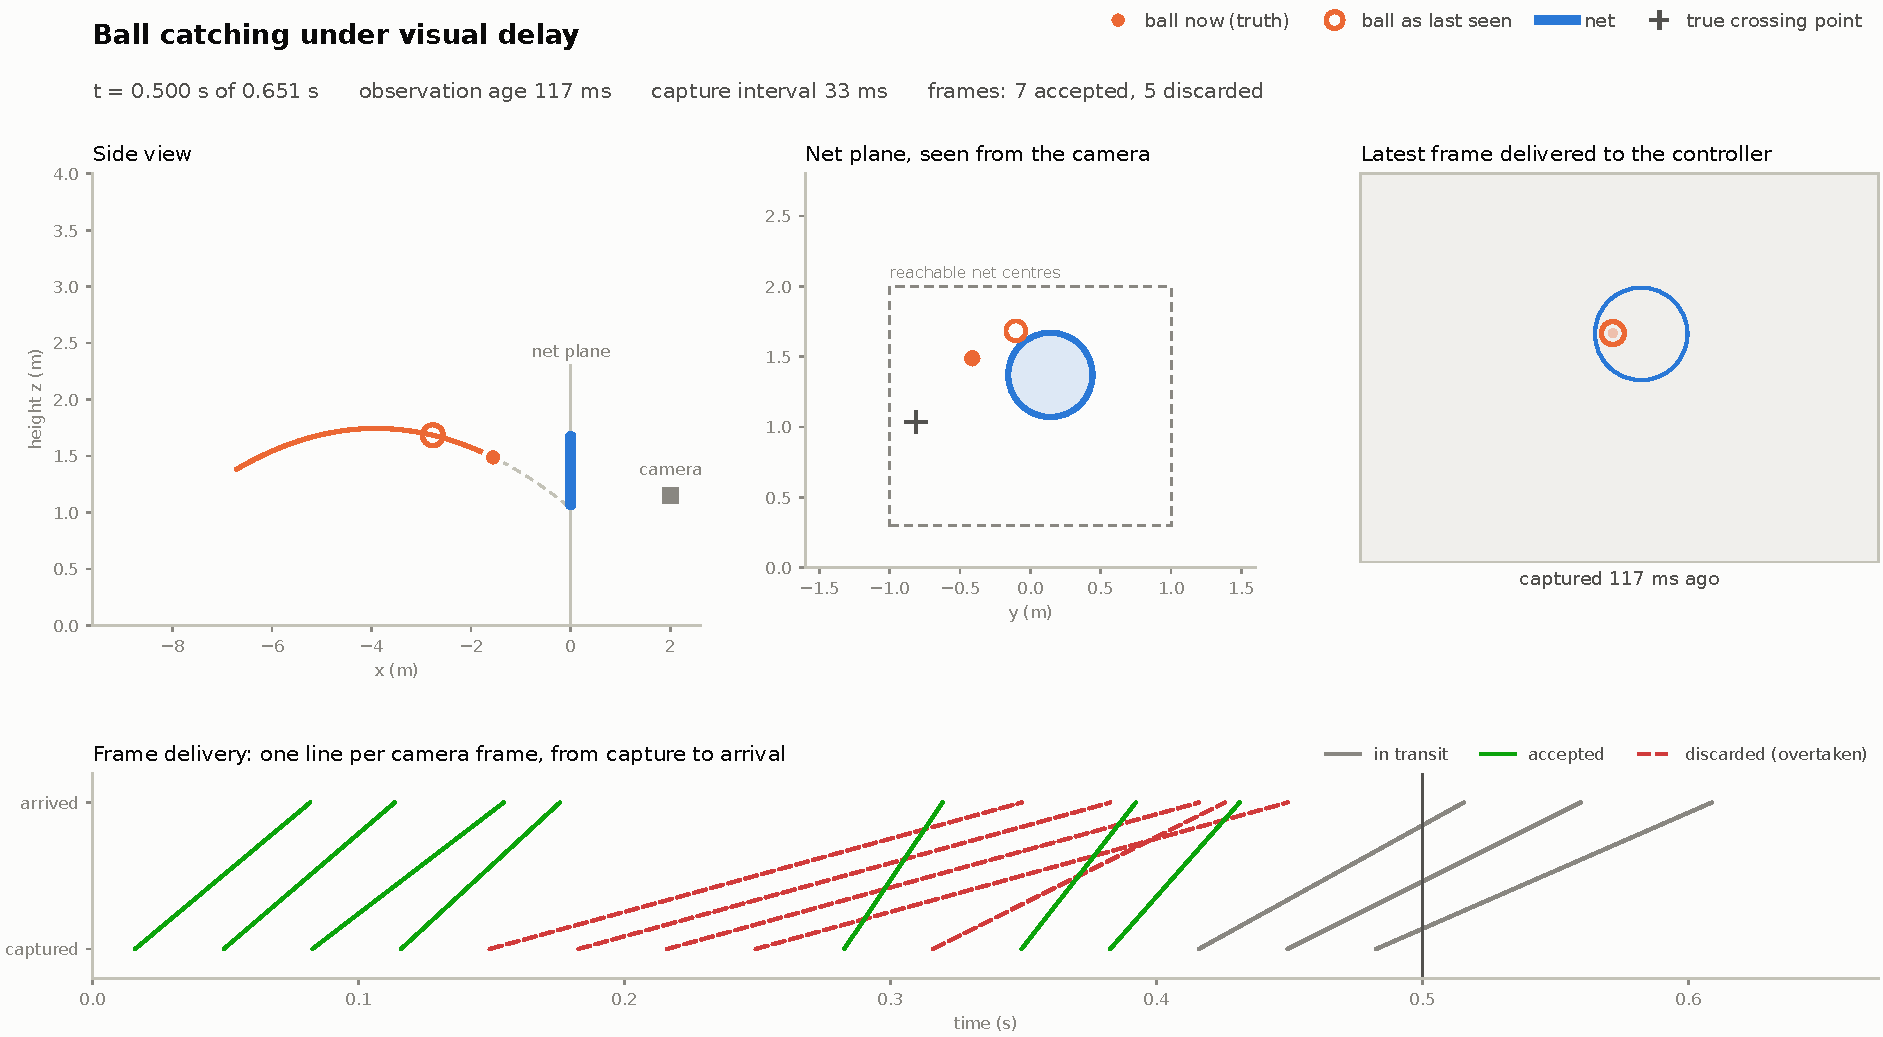
\includegraphics[width=0.88\textwidth]{figures/render.pdf}
  \caption{Visualisation, from \code{python demo.py -{}-delay burst -{}-seed 3} at $t = 0.5$\,s.
    Filled dot: the true ball. Hollow ring: where the controller last saw it. Bottom: one line per
    camera frame, from capture to arrival; red dashed frames were overtaken by newer ones and
    discarded. Here a stall of four frames leaves the controller with a 117\,ms old view.}
  \label{fig:render}
\end{figure}

%==========================================================================================
\section{Existing Codes and Libraries}

We did not use a robot simulator, and we did not copy code from online sources. The environment was
written for this project with the help of AI coding assistants (see the declaration at the end).
\begin{itemize}
  \item \textbf{Gym 0.26.2}: the \code{gym.Env} base class, \code{spaces.Box}, registration and the
        environment checker. It is the course's reference version, so we follow its API: \code{reset}
        returns \code{(obs, info)} and \code{step} returns five values. The older Gym 0.23 on our machine
        expects four, so we set up a clean environment pinned to 0.26.2 (\code{environment.yml}).
  \item \textbf{NumPy 1.23.5}: maths and random numbers. Gym 0.26.2 does not support NumPy 2, so we pin
        a 1.x version. All randomness comes from the generator Gym seeds in \code{reset(seed=...)}, so
        any episode can be replayed exactly.
  \item \textbf{Matplotlib 3.7.5} for the visualisation, \textbf{Pillow} for GIFs. \code{rgb\_array} mode
        draws off-screen, so it needs no display. Newer Pillow and pyparsing make this Matplotlib print
        warnings, so we pin them to 10.4.0 and 3.1.4.
  \item Python standard library: \code{heapq} for the frame queue, \code{unittest} and \code{argparse}.
\end{itemize}
\textbf{Why no physics simulator?} The ball follows a parabola we can compute exactly, and we do not
simulate contact with the net, so a simulator such as PyBullet would add little. Writing it ourselves
gives exact control over \emph{when} each frame is captured and delivered, which is the core of our
study. The price was building our own visualisation.

%==========================================================================================
\section{Reflections and Lessons Learned}

\textbf{Changes from the proposal.}
\begin{itemize}
  \item \textbf{Concrete timing (TA feedback).} Flight 0.6--1.2\,s; camera 30\,Hz (18--36 frames per
        throw); control 60\,Hz; maximum delay 0.2\,s, which is 17--33\% of the flight.
  \item \textbf{Net limits from a pilot calibration (TA feedback).} Our first guess, 10\,m/s$^2$, was
        too generous: an oracle starting 0.27\,s late still caught 97\% of balls, so delay hardly
        mattered. With 6\,m/s$^2$ (the 3\,m/s cap is never reached), catching is feasible, not trivial,
        and sensitive to delay when there is little time to recover (Table~\ref{tab:calibration}).
  \item \textbf{Distance-based reward (TA feedback).} The proposal gave $+1$ or $-1$. Now a catch near
        the centre earns more, and a near miss costs less than a large miss. A catch still beats any
        miss by at least 1.
  \item \textbf{Simplifications.} Circular net; noisy pinhole features, not rendered images; the ball is
        always in view, so the detection flag stays 1.
  \item \textbf{Rules we pinned down.} If several frames arrive in one step, only the newest is accepted.
        Throws are built from a chosen flight time and crossing point, so difficulty is easy to control.
\end{itemize}

\begin{table}[h!]
  \centering
  \caption{Pilot calibration: success rate over the same 1,000 throws (\code{python calibrate.py}).
    \emph{Chase} follows the line of sight to the last seen ball. \emph{Oracle} knows the true crossing
    point but only starts moving after the delay plus two camera frames.}
  \label{tab:calibration}
  \small
  \begin{tabular}{@{}lcccc@{}}
    \toprule
    Fixed delay & Stationary net & Chase & Oracle, all throws & Oracle, flights $<$ 0.8\,s \\
    \midrule
    0       & 5.1\% & 18.8\% & 100.0\% & 100.0\% \\
    0.10\,s & 5.1\% & 10.8\% &  95.8\% &  86.6\% \\
    0.20\,s & 5.1\% &  8.0\% &  88.0\% &  62.0\% \\
    \bottomrule
  \end{tabular}
\end{table}

\textbf{Lessons learned.}
\begin{itemize}
  \item \textbf{Check that delay matters before training.} Hand-written controllers showed this in minutes.
  \item \textbf{Delay also means lost frames.} With $80 \pm 40$\,ms jitter, 36\% of frames are overtaken and
        discarded, leaving about 19 of 30 per second.
  \item \textbf{Reacting is not enough.} The chase policy catches only 19\% even without delay: on high,
        slow throws the line of sight pulls the net up too early. This supports using memory and
        prediction.
\end{itemize}

\textbf{Next steps.} Train the PPO variants; build the predictive baseline; tune $\lambda$ on held-out seeds; run the stall tests.

\textbf{AI tool declaration.} We used Claude and GPT, through the AI assistant, to help design, write and
test the environment code, and optimize the report. The requirements for the project were
proposed by us after discussion. We are responsible for the content and quality of the submitted work.

\end{document}
